\documentclass[../main.tex]{subfiles}
\providecommand{\main}{..}
\def\biblio{\addbibresource{\main/main.bib}}
%\biblio
%\addbibresource{\main/main.bib}

\begin{document}

The Office of Advancement gave us four password protected Microsoft Excel
files, Bio.csv, Events.csv, Actions.csv, and Gifts.csv. The college has been
collecting biographical information on potential donors and event attendees.
In Bio.csv, each row is contains a person's identification number along with
that person's biographical information. The labels for this file are below:

\vline

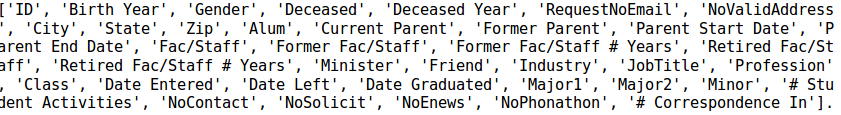
\includegraphics[width=10cm, height=3cm]{bio_titles.png}

\vline

The identification number used in Bio.csv can be used to obtain information
about that person's event attendance, donation history, and how that person
has been contacted over time. Each row in Events.csv records an instance of
someone attending some event on some date, and each row in Gifts.csv records
an instance of someone or some organization donating some amount of money on
same date. The most interesting file for this analysis is Actions.csv. The
college can contact someone by email, phone, meeting, or mailing, and the
college records each time it contacts someone as a row in Actions.csv, where
the row contains the id of the person being contacted, how the person was
contacted, and on what date the person was contacted. The file does not
contain mass emails which are frequently sent out or the biannual Phonathon
event; however, this file, which has been recorded since April 30, 2002,
provides pretty useful information. Since the focus of this project was how
actions could be altered, we only included data during the time frame during
which data about actions was available. To do this, we sorted Events.csv,
Gifts.csv, and Actions.csv by date and removed any rows in these files that
had dates preceding the start of Actions.csv. These files were exported as
csvs and data analysis was performed in an Ipython notebook, which is stored
in this directory.

\end{document}
